% !TeX spellcheck = <english>
\documentclass{beamer}
%\documentclass[aspectratio=169]{beamer}

% You have to install the theme first!

% corporate design of TU Wien
\usetheme[font=futura]{tuw}
% background "TU main building" on title page
%\usetheme[tuw_background]{tuw}
% individual background on title page
%\usetheme[tuw_image=TU_Background]{tuw}
% white logo if you have a dark background image
%\usetheme[tuw_image=TU_Background,tuw_whitelogo]{tuw}
% sidebar (not in TU Wien CD! but nice for long presentations)
% width of the sidebar can be changed with option: "width=2cm"
%\usetheme[outer=sidebar]{tuw}
% move frametitle up (beside logo)
%\usetheme[tuw_frametitletotop]{tuw}

% if you use german umlaute use T1 encoding:
%\usepackage[T1]{fontenc}
% default Latex fonts are not T1 supported -> bitmaps used, this is not nice on
% screen; you can use the lmodern package instead
%\usepackage{lmodern}
\usepackage[utf8]{inputenc}
\usepackage{listings}
\usepackage{booktabs}
\usepackage{url}
\usepackage{apacite}
\usepackage{tikz,pgfplots}
\usepackage{mathtools}

\pgfplotsset{compat=1.7}
\bibliographystyle{apacite}
\DeclarePairedDelimiter\norm{\lVert}{\rVert}

%%% title page settings
\title[Affinity Propagation]{%
  Clustering with Affinity Propagation
}
\subtitle{...and its Applications}
\author{Philipp-Alexander Auer}
\date{\today}


%%% slides start here
\begin{document}

% first frame must include the title page!
\begin{frame}
  \titlepage
\end{frame}

% table of contents if you have a long presentation (uses 'part' and 'section'
% elements)
\begin{frame}{Outline}
  \tableofcontents
\end{frame}

\section{Clustering}

\subsection[Overview]{Overview}
\begin{frame}[fragile]
  \frametitle{Clustering: Overview\footnote{\cite{kaufman2009finding}}}
  \begin{itemize}
  	\item Cluster Analysis is the art of finding groups in data. 
  	\item To do so, we need to specify a similarity criterion (e.g. the euclidian distance as a metric)
  	\item We want to automatize this clustering process.
  	
  \end{itemize}
\end{frame}
\begin{frame}[fragile]
\frametitle{Clustering: Overview}
\begin{figure}
	\centering
	\scalebox{0.65}{
		% This file was created by tikzplotlib v0.8.5.
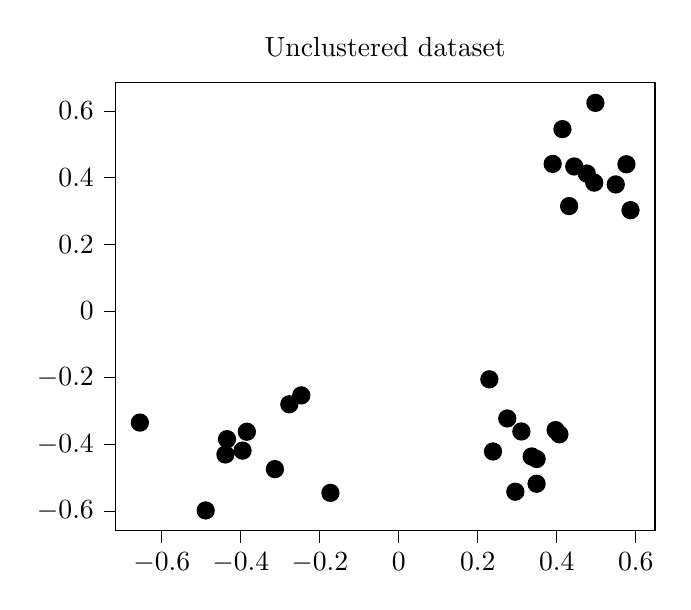
\begin{tikzpicture}

\begin{axis}[
tick align=outside,
tick pos=left,
title={Unclustered dataset},
x grid style={white!69.01960784313725!black},
xmin=-0.717401720613328, xmax=0.648858538044917,
xtick style={color=black},
y grid style={white!69.01960784313725!black},
ymin=-0.65918809515952, ymax=0.685197768257273,
ytick style={color=black}
]
\addplot [semithick, black, mark=*, mark size=3, mark options={solid}, only marks]
table {%
0.414404357116088 0.545427350696298
};
\addplot [semithick, black, mark=*, mark size=3, mark options={solid}, only marks]
table {%
-0.438732681740795 -0.430230275057534
};
\addplot [semithick, black, mark=*, mark size=3, mark options={solid}, only marks]
table {%
-0.395424148269855 -0.418718385002583
};
\addplot [semithick, black, mark=*, mark size=3, mark options={solid}, only marks]
table {%
-0.488778574763011 -0.598079646822393
};
\addplot [semithick, black, mark=*, mark size=3, mark options={solid}, only marks]
table {%
-0.173024537601239 -0.545436567459876
};
\addplot [semithick, black, mark=*, mark size=3, mark options={solid}, only marks]
table {%
-0.313556380114049 -0.474216502040644
};
\addplot [semithick, black, mark=*, mark size=3, mark options={solid}, only marks]
table {%
0.444386323274543 0.433367432737427
};
\addplot [semithick, black, mark=*, mark size=3, mark options={solid}, only marks]
table {%
0.576405234596766 0.440015720836722
};
\addplot [semithick, black, mark=*, mark size=3, mark options={solid}, only marks]
table {%
0.295144703493291 -0.542001793717898
};
\addplot [semithick, black, mark=*, mark size=3, mark options={solid}, only marks]
table {%
0.348919486243113 -0.518063218412241
};
\addplot [semithick, black, mark=*, mark size=3, mark options={solid}, only marks]
table {%
0.549407907315761 0.37948417362342
};
\addplot [semithick, black, mark=*, mark size=3, mark options={solid}, only marks]
table {%
0.476103772514699 0.412167501649283
};
\addplot [semithick, black, mark=*, mark size=3, mark options={solid}, only marks]
table {%
-0.384505257430308 -0.362183748039783
};
\addplot [semithick, black, mark=*, mark size=3, mark options={solid}, only marks]
table {%
0.389678114820644 0.441059850193837
};
\addplot [semithick, black, mark=*, mark size=3, mark options={solid}, only marks]
table {%
0.497873798410574 0.624089319920146
};
\addplot [semithick, black, mark=*, mark size=3, mark options={solid}, only marks]
table {%
-0.655298981583408 -0.334638140455964
};
\addplot [semithick, black, mark=*, mark size=3, mark options={solid}, only marks]
table {%
0.43130677016509 0.314590426069828
};
\addplot [semithick, black, mark=*, mark size=3, mark options={solid}, only marks]
table {%
0.229372980937499 -0.204922460476821
};
\addplot [semithick, black, mark=*, mark size=3, mark options={solid}, only marks]
table {%
0.349034781824835 -0.443807430161119
};
\addplot [semithick, black, mark=*, mark size=3, mark options={solid}, only marks]
table {%
-0.434791214932615 -0.384365103089602
};
\addplot [semithick, black, mark=*, mark size=3, mark options={solid}, only marks]
table {%
0.336567790631904 -0.436274116598714
};
\addplot [semithick, black, mark=*, mark size=3, mark options={solid}, only marks]
table {%
-0.246722078564154 -0.253064123009971
};
\addplot [semithick, black, mark=*, mark size=3, mark options={solid}, only marks]
table {%
-0.276970931927228 -0.279762015121559
};
\addplot [semithick, black, mark=*, mark size=3, mark options={solid}, only marks]
table {%
0.238610215244205 -0.421274028021397
};
\addplot [semithick, black, mark=*, mark size=3, mark options={solid}, only marks]
table {%
0.495008841752559 0.38486427917023
};
\addplot [semithick, black, mark=*, mark size=3, mark options={solid}, only marks]
table {%
0.406651722238317 -0.369752810226022
};
\addplot [semithick, black, mark=*, mark size=3, mark options={solid}, only marks]
table {%
0.310453343880632 -0.361309750214074
};
\addplot [semithick, black, mark=*, mark size=3, mark options={solid}, only marks]
table {%
0.586755799014997 0.302272212012359
};
\addplot [semithick, black, mark=*, mark size=3, mark options={solid}, only marks]
table {%
0.397181777166135 -0.357166812946958
};
\addplot [semithick, black, mark=*, mark size=3, mark options={solid}, only marks]
table {%
0.274720463995007 -0.322250964416809
};
\end{axis}

\end{tikzpicture}

	}
	\caption{3 clusters, unclustered dataset}
	\label{fig:unclust}
\end{figure}
\end{frame}

\begin{frame}[fragile]
\frametitle{Clustering: Overview}
\begin{figure}
	\centering
	\scalebox{0.65}{
		% This file was created by tikzplotlib v0.8.5.
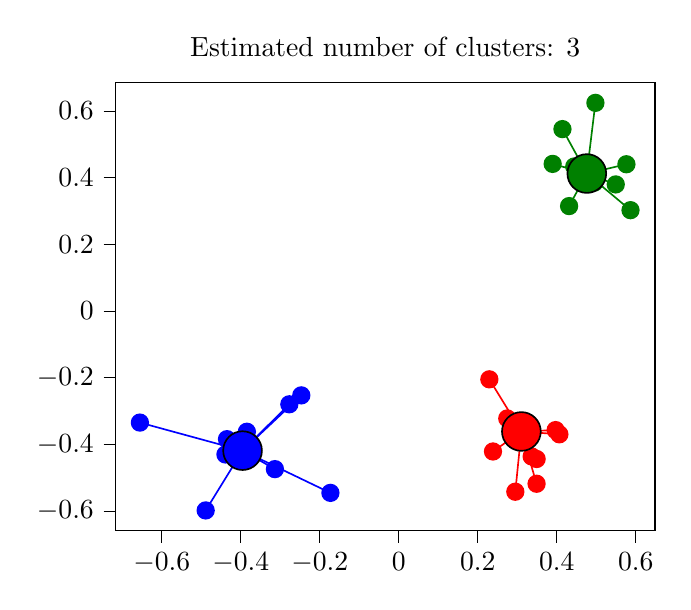
\begin{tikzpicture}

\definecolor{color0}{rgb}{0.12156862745098,0.466666666666667,0.705882352941177}
\definecolor{color1}{rgb}{1,0.498039215686275,0.0549019607843137}
\definecolor{color2}{rgb}{0.172549019607843,0.627450980392157,0.172549019607843}

\begin{axis}[
tick align=outside,
tick pos=left,
title={Estimated number of clusters: 3},
x grid style={white!69.01960784313725!black},
xmin=-0.717401720613328, xmax=0.648858538044917,
xtick style={color=black},
y grid style={white!69.01960784313725!black},
ymin=-0.65918809515952, ymax=0.685197768257273,
ytick style={color=black}
]
\addplot [semithick, blue, mark=*, mark size=3, mark options={solid}, only marks]
table {%
-0.438732681740795 -0.430230275057534
-0.395424148269855 -0.418718385002583
-0.488778574763011 -0.598079646822393
-0.173024537601239 -0.545436567459876
-0.313556380114049 -0.474216502040644
-0.384505257430308 -0.362183748039783
-0.655298981583408 -0.334638140455964
-0.434791214932615 -0.384365103089602
-0.246722078564154 -0.253064123009971
-0.276970931927228 -0.279762015121559
};
\addplot [semithick, color0, mark=*, mark size=7, mark options={solid,fill=blue,draw=black}, only marks]
table {%
-0.395424148269855 -0.418718385002583
};
\addplot [semithick, blue]
table {%
-0.395424148269855 -0.418718385002583
-0.438732681740795 -0.430230275057534
};
\addplot [semithick, blue]
table {%
-0.395424148269855 -0.418718385002583
-0.395424148269855 -0.418718385002583
};
\addplot [semithick, blue]
table {%
-0.395424148269855 -0.418718385002583
-0.488778574763011 -0.598079646822393
};
\addplot [semithick, blue]
table {%
-0.395424148269855 -0.418718385002583
-0.173024537601239 -0.545436567459876
};
\addplot [semithick, blue]
table {%
-0.395424148269855 -0.418718385002583
-0.313556380114049 -0.474216502040644
};
\addplot [semithick, blue]
table {%
-0.395424148269855 -0.418718385002583
-0.384505257430308 -0.362183748039783
};
\addplot [semithick, blue]
table {%
-0.395424148269855 -0.418718385002583
-0.655298981583408 -0.334638140455964
};
\addplot [semithick, blue]
table {%
-0.395424148269855 -0.418718385002583
-0.434791214932615 -0.384365103089602
};
\addplot [semithick, blue]
table {%
-0.395424148269855 -0.418718385002583
-0.246722078564154 -0.253064123009971
};
\addplot [semithick, blue]
table {%
-0.395424148269855 -0.418718385002583
-0.276970931927228 -0.279762015121559
};
\addplot [semithick, green!50.0!black, mark=*, mark size=3, mark options={solid}, only marks]
table {%
0.414404357116088 0.545427350696298
0.444386323274543 0.433367432737427
0.576405234596766 0.440015720836722
0.549407907315761 0.37948417362342
0.476103772514699 0.412167501649283
0.389678114820644 0.441059850193837
0.497873798410574 0.624089319920146
0.43130677016509 0.314590426069828
0.495008841752559 0.38486427917023
0.586755799014997 0.302272212012359
};
\addplot [semithick, color1, mark=*, mark size=7, mark options={solid,fill=green!50.0!black,draw=black}, only marks]
table {%
0.476103772514699 0.412167501649283
};
\addplot [semithick, green!50.0!black]
table {%
0.476103772514699 0.412167501649283
0.414404357116088 0.545427350696298
};
\addplot [semithick, green!50.0!black]
table {%
0.476103772514699 0.412167501649283
0.444386323274543 0.433367432737427
};
\addplot [semithick, green!50.0!black]
table {%
0.476103772514699 0.412167501649283
0.576405234596766 0.440015720836722
};
\addplot [semithick, green!50.0!black]
table {%
0.476103772514699 0.412167501649283
0.549407907315761 0.37948417362342
};
\addplot [semithick, green!50.0!black]
table {%
0.476103772514699 0.412167501649283
0.476103772514699 0.412167501649283
};
\addplot [semithick, green!50.0!black]
table {%
0.476103772514699 0.412167501649283
0.389678114820644 0.441059850193837
};
\addplot [semithick, green!50.0!black]
table {%
0.476103772514699 0.412167501649283
0.497873798410574 0.624089319920146
};
\addplot [semithick, green!50.0!black]
table {%
0.476103772514699 0.412167501649283
0.43130677016509 0.314590426069828
};
\addplot [semithick, green!50.0!black]
table {%
0.476103772514699 0.412167501649283
0.495008841752559 0.38486427917023
};
\addplot [semithick, green!50.0!black]
table {%
0.476103772514699 0.412167501649283
0.586755799014997 0.302272212012359
};
\addplot [semithick, red, mark=*, mark size=3, mark options={solid}, only marks]
table {%
0.295144703493291 -0.542001793717898
0.348919486243113 -0.518063218412241
0.229372980937499 -0.204922460476821
0.349034781824835 -0.443807430161119
0.336567790631904 -0.436274116598714
0.238610215244205 -0.421274028021397
0.406651722238317 -0.369752810226022
0.310453343880632 -0.361309750214074
0.397181777166135 -0.357166812946958
0.274720463995007 -0.322250964416809
};
\addplot [semithick, color2, mark=*, mark size=7, mark options={solid,fill=red,draw=black}, only marks]
table {%
0.310453343880632 -0.361309750214074
};
\addplot [semithick, red]
table {%
0.310453343880632 -0.361309750214074
0.295144703493291 -0.542001793717898
};
\addplot [semithick, red]
table {%
0.310453343880632 -0.361309750214074
0.348919486243113 -0.518063218412241
};
\addplot [semithick, red]
table {%
0.310453343880632 -0.361309750214074
0.229372980937499 -0.204922460476821
};
\addplot [semithick, red]
table {%
0.310453343880632 -0.361309750214074
0.349034781824835 -0.443807430161119
};
\addplot [semithick, red]
table {%
0.310453343880632 -0.361309750214074
0.336567790631904 -0.436274116598714
};
\addplot [semithick, red]
table {%
0.310453343880632 -0.361309750214074
0.238610215244205 -0.421274028021397
};
\addplot [semithick, red]
table {%
0.310453343880632 -0.361309750214074
0.406651722238317 -0.369752810226022
};
\addplot [semithick, red]
table {%
0.310453343880632 -0.361309750214074
0.310453343880632 -0.361309750214074
};
\addplot [semithick, red]
table {%
0.310453343880632 -0.361309750214074
0.397181777166135 -0.357166812946958
};
\addplot [semithick, red]
table {%
0.310453343880632 -0.361309750214074
0.274720463995007 -0.322250964416809
};
\end{axis}

\end{tikzpicture}

	}
	\caption{3 clusters, clustered and colorized dataset}
	\label{fig:clust}
\end{figure}
\end{frame}

\subsection[classical]{Algorithms}
\begin{frame}
  \frametitle{Clustering: Algorithms}
  Many algorithms exist to solve the clustering problem, one of the more popular ones is \emph{k-means}. \cite{frey2007clustering}
  
  This presentation / paper shall discuss \emph{Affinity Propagation} proposed by \cite{frey2007clustering}. 
\end{frame}

\section{Affinity Propagation}
\subsection{How it works}
\begin{frame}{Affinity Propagation\footnote{\cite{frey2007clustering}}: Overview}
	AP can find clusters and their respective \alert{exemplars} (Data points, which act as the center of a cluster, see Figure \ref{fig:clust})
	
	AP takes as input the \alert{similarity matrix} $s(i,k)$.
	
	In each step, AP updates the message matrices $r(i,k)$ (\alert{responsiblity matrix}) and $a(i,k)$ (\alert{availability matrix})
	
	Message passing may be terminated at any time, e.g. after:
	\begin{itemize}
		\item Fixed amount of iterations
		\item Changes fall below a threshold
		\item Local decisions stay constant for some number of iterations
	\end{itemize}
\end{frame}

\begin{frame}{Affinity Propagation: Similarity Matrix}
	Initially, the \alert{similarity matrix} has to be set. $s(i,k)$ indicates how suited data point $k$ is to be an \alert{exemplar} for data point $i$.
	
	Often you want to use a metric, e.g. the negative squared error (\alert{Euclidean distance})
	
	\begin{block}{Negative squared error}
		\begin{center}
			$s(i,k) = -\norm{x_i - x_k}^2$
		\end{center}
	\end{block}
\end{frame}

\begin{frame}{Affinity Propagation: Similarity Matrix}
    AP does not need a specified number of clusters.
    
    Instead it takes the so-called \alert{preference values} $s(k,k)$ as an input, that describe the log-likelihood of $x_k$ being an \alert{exemplar}.
    
    If each point is equally likely to be an \alert{exemplar}, this can be set to a common value $s(k,k) = p$. Frey et al. suggest to use the similarity median for `p`
\end{frame}

\begin{frame}{Affinity Propagation: Responsibility Matrix}
	To begin, the \alert{availability matrix} is initialized to $a(i,k) = 0$.
	
	The \alert{responsibility} $r(i,k)$ sent from point $i$ to point $k$ reflects how suited point $k$ is to serve as an \alert{exemplar} for point $i$. It is updated in each step:
	
	\begin{block}{Updating the responsibility}
		\begin{center}
			$r(i,k) \leftarrow s(i,k) - \underset{k^\prime\, \mathsf{s.t.}\, k^\prime \neq k}{\mathsf{max}} \{a(i,k^\prime) + s(i,k^\prime)\}$
		\end{center}
	\end{block}
\end{frame}

\begin{frame}{Affinity Propagation: Availability Matrix}
    The \alert{availability} $a(i,k)$ sent from candidate \alert{exemplar} $k$ to point $i$ reflects how appropriate it would be for point $i$ to choose $k$ as its \alert{exemplar}. It is updated after the new \alert{responsibility matrix} is calculated:
    
    \begin{block}{Updating the availability}
		\begin{center}
			$a(i,k) \leftarrow \mathsf{min}\{0,r(k,k) + \sum\limits_{i^\prime\,\mathsf{s.t.}\, i^\prime \notin \{i,k\}}\mathsf{max}\{0, r(i^{\, \prime} ,k)\}\}$
		\end{center}
    \end{block}
	Negative portions of incoming \alert{responsibilities} are ignored, because a good \alert{exemplar} only needs to explain some datapoints well.
\end{frame}

\begin{frame}{Affinity Propagation: Self-Availability}
    The "\alert{self-availability}" $a(k,k)$ reflects accumulated evidence that point $k$ is an \alert{exemplar}, based on positive \alert{responsibilities} sent to $k$ from other points. It is updated differently:
    
    \begin{block}{Updating the self-availability}
    	\begin{center}
    		$a(k,k) \leftarrow \sum\limits_{i^\prime\, \mathsf{s.t.}\, i^\prime \neq k} \mathsf{max} \{0, r(i^{\, \prime} ,k)\}$
    	\end{center}
    \end{block}
\end{frame}

\begin{frame}{Affinity Propagation: Gathering Clusters}
	After the message passing terminates, \alert{availabilities} and \alert{respnsibilities} can be combined to identify \alert{exemplars} and clusters.
	
	The value that maximizes $a(i,k) + r(i,k)$ eighter identifies point $i$ as an \alert{exemplar} if $i=k$ or identifies the data point that is the \alert{exemplar} for point $i$.
\end{frame}
\begin{frame}{Affinity Propagation: Oscillations}
	In order to reduce numerical oscillations in the message-passing process, a damping factor $\lambda$ shall be used:
	\begin{block}{Updating with a damping factor}
		\begin{center}
			$M(i,j) =\lambda M(i,j) + (1-\lambda) M^\prime (i,j)$
		\end{center}
	\end{block}
	 for message matrix $M$ and $\lambda\in\left[ 0,1\right]$.
	
	The damping factor can be chosen arbitrarily to suit the given dataset / expexted outcome. Default: $\lambda = 0.5$.
\end{frame}

\subsection{Differences to classical algorithms}
\begin{frame}{Affinity Propagation: Differences to classical algorithms}
	\begin{itemize}
		\item AP does not need a specified amount of clusters.
		\begin{itemize}
			\item They emerge from the preference and message-passing.
		\end{itemize}
		\item AP does not need a metric.
		\begin{itemize}
			\item The \alert{similarity matrix} can take any real values, and does not need to be symmetric.
		\end{itemize}
		\item Because of its nature the user needs to play around with the \alert{preference values} and \alert{damping factor} in order to achieve a suitable outcome.
	\end{itemize}
\end{frame}

\subsection{Examples}
\begin{frame}{Affinity Propagation: Example}
	\begin{center}
		Video of AP clustering plotted for different iterations
	\end{center}
\end{frame}

\subsection{Problems}
\begin{frame}{Affinity Propagation: Problems}
	The matrices tend to oscillate a lot, which can lead to long (if ever) convergence times. \cite{frey2007clustering} 
	
	To deal with that the damping factor $\lambda$ can be used, and preferences can be set accordingly, but its hard to predict exactly what preference values work best. \cite{wang2008adaptive}
	
	An adapted algorithm was proposed by Wang et al. - Called Adaptive Affinity Propagation, which adjusts damping factors to escape oscillations. \cite{wang2008adaptive}
\end{frame}
\begin{frame}{Overcoming Oscillations: Adaptive AP\footnote{\cite{wang2008adaptive}}}
	A high $\lambda$ will get rid of oscillations, but also slows down message passing.
	
	Wang et al. propose an adaptive way to update $\lambda = \lambda+0.05$ if oscillations are detected. A sliding window of size $w$ keeps track of previous values in the message passing.
	
	If $\lambda$ reaches a treshold of $0.85$, $p$ is also increased by $p_\Delta$ to escape oscillations.
\end{frame}
\subsection{Applications}
\begin{frame}{Affinity Propagation}{Applications}
	Frey et al. tried their algorithm on clustering for face images, genes, sentences and airline travel routes, which worked rather well compared to traditional algorithms. \cite{frey2007clustering}
	
	Other people have since tried to use AP for a number of different approaches, e.g. fingerprint-based WLAN positioning, as proposed by Tian et al. \cite{tian2013fingerprint}
\end{frame}
\begin{frame}{Applications: WLAN fingerprinting\footnote{\cite{tian2013fingerprint}}}
	Tian et al. combine AP clustering with probability based indoor positioning.
	
	Their algorithm clusters the \alert{Received Signal Strength} before applying a probability based algorithm.
	
	Reduces computation time and errors, because only the cluster's \alert{Exemplar} is used as a reference point.
\end{frame}
\begin{frame}{Thank you}
	Thank you for your attention, for a complete list of results please consider viewing the references.
	
	Feel free to ask questions. :)
\end{frame}
\begin{frame}{References}
	\bibliography{../literature/literature}
\end{frame}
\end{document}
